\documentclass[letterpaper]{scrartcl}	
\usepackage[top=0.88in, bottom=1in, left=1in, right=1in]{geometry}

\makeatletter
\DeclareOldFontCommand{\tt}{\normalfont\ttfamily}{\mathtt}
\makeatother

\usepackage{scalefnt}
\usepackage{bm}
\usepackage{cancel}

%--------------------------------------------------------------
% We need this package, part of the KOMA class, for the custom
% headings.
%--------------------------------------------------------------
\usepackage{scrpage2}	
		

%--------------------------------------------------------------
% One of many packages you can use if you want to include
% graphics.
%--------------------------------------------------------------
\usepackage{graphicx}			

%--------------------------------------------------------------
% The AMS packages are useful but not required. They offer a
% number of nice fonts, environments for formatting multiline
% equations, etc.
%--------------------------------------------------------------
\usepackage{amsmath}			
\usepackage{amsfonts}
\usepackage{amssymb}
\usepackage{amsthm}

%--------------------------------------------------------------
% Basic way to set-up the page margins.
%--------------------------------------------------------------
%\addtolength{\oddsidemargin}{-.2in}
%\addtolength{\evensidemargin}{-.2in}
%\addtolength{\textwidth}{0.45in}
%\addtolength{\topmargin}{-.175in}
%\addtolength{\textheight}{0.75in}

%--------------------------------------------------------------
% Comment out the following to add indents and remove space between paragraphs.
%--------------------------------------------------------------
\usepackage{parskip}

%--------------------------------------------------------------
% This package is used to define custom colours.
%--------------------------------------------------------------
\usepackage[usenames,dvipsnames,svgnames,table]{xcolor}

%--------------------------------------------------------------
% Package for adding in solutions:
%--------------------------------------------------------------
\usepackage[nosoln,regf,nolf]{optional}
%\usepackage[soln,regf]{optional}

%\newcommand{\soln}[1]{\opt{soln}{\\[4pt] \textcolor{JungleGreen}{\textbf{Solution:}} #1}}
\newcommand{\soln}[1]{\opt{soln}{\textcolor{JungleGreen}{\usekomafont{descriptionlabel}{Solution:}} #1}}

\newcommand{\hint}[1]{{\usekomafont{descriptionlabel}{Hint:}} #1}
\newcommand{\note}[1]{{\usekomafont{descriptionlabel}{Note:}} #1}
\newcommand{\reference}[1]{{\usekomafont{descriptionlabel}{Reference:}} #1}

%--------------------------------------------------------------
% A few colours for hyperlinks.
%--------------------------------------------------------------
\definecolor{plum}{rgb}{0.36078, 0.20784, 0.4}
\definecolor{chameleon}{rgb}{0.30588, 0.60392, 0.023529}
\definecolor{cornflower}{rgb}{0.12549, 0.29020, 0.52941}
\definecolor{scarlet}{rgb}{0.8, 0, 0}
\definecolor{brick}{rgb}{0.64314, 0, 0}

%--------------------------------------------------------------
% A command for typesetting and linking an email address.
%--------------------------------------------------------------
\newcommand{\email}[1]{\href{mailto:#1}{\tt \textcolor{cornflower}{#1}}}
\newcommand{\web}[1]{\href{#1}{\tt \textcolor{cornflower}{#1}}}

%--------------------------------------------------------------
%  The following declaration includes the hyperref package and
% assigns metadata. If you compile with pdflatex, this data
% will be automatically included in the pdf file.
%--------------------------------------------------------------
%\usepackage[
%	pdftitle={QFT Tutorial 1},%
%	pdfauthor={PSI Tutors},%
%	pdfsubject={QFT Tutorial 1},%
%	pdfkeywords={PSI},
%	colorlinks=true,
%	linkcolor=cornflower,
%	citecolor=scarlet,
%	urlcolor=chameleon%
%]{hyperref}

%\setcounter{secnumdepth}{2}	% section number depth
%\setcounter{tocdepth}{2}		% depth of TOC

%--------------------------------------------------------------
% Specify the font used in captions.
%--------------------------------------------------------------
\setkomafont{captionlabel}{\usekomafont{descriptionlabel}}

%--------------------------------------------------------------
% This is where we define the custom title. The image that is
% placed on the left-hand-side of the title, PILogo.pdf in
% this case, should be in the same directory as this file. Note
% that you can always use hyperlinks for the Title, Semester,
% and Author fields, below, in case you want to link to a seminar
% web page or a lecturer's email address.
%--------------------------------------------------------------

%\titlehead{%
%	\vspace*{-1cm}
%	\begin{minipage}[b]{4.0cm}
%	\includegraphics*[height=1.3cm]{PSIletterhead.eps}%
%	\end{minipage}
%	\hfill
%	\begin{minipage}[b]{10cm}
%%	\begin{flushright}
	%	\usekomafont{descriptionlabel}
	%	\Large Machine Learning for Many-Body Physics \\
	%	\normalsize \normalfont Spring 2019\\
	%	Lauren Hayward Sierens
	%\end{flushright}
%	\end{minipage}
%	\\[-3mm]
%	\hrule
%	\vspace{-3mm}
%}
% -----------
\titlehead{%
	\vspace*{-1cm}
	\begin{minipage}[b]{4.0cm}
	\includegraphics*[height=1.3cm]{Uniandes_logo.jpeg}%
	\end{minipage}
	\hfill
	\begin{minipage}[b]{12cm}
	\begin{flushright}
		\usekomafont{descriptionlabel}
		\large Machine Learning for Quantum Matter and Technology \\
		\normalsize \normalfont
		J. Carrasquilla, E. Inack, G. Torlai, R. Melko, L. Hayward Sierens
	\end{flushright}
	\end{minipage}
	\\[-3mm]
	\hrule
	\vspace{-3mm}
}

%--------------------------------------------------------------
% Other useful physic-related packages
%--------------------------------------------------------------
\usepackage{braket}  
% Use \Bra{}, \Ket{} or \Braket{x | \psi} for Dirac notation

%--------------------------------------------------------------
% Nice numbering for question parts.
%--------------------------------------------------------------
\newcommand{\ba}{\begin{eqnarray}}
\newcommand{\ea}{\end{eqnarray}}

\newcommand{\ssk}{\smallskip}
\newcommand{\msk}{\medskip}

\newcommand{\nin}{\noindent}

\newcommand{\beq}{\begin{equation}}
\newcommand{\eeq}{\end{equation}}

\newcommand{\beqs}{\begin{equation*}}
\newcommand{\eeqs}{\end{equation*}}

\renewcommand{\vec}[1]{{\mathbf{#1}}}
\renewcommand{\labelenumi}{\alph{enumi})}
\renewcommand{\labelenumiii}{\roman{enumiii})}

%%%%%%%%%%%%%

\def\be{\begin{eqnarray}}
\def\ee{\end{eqnarray}}
\newcommand{\nn}{\nonumber}
\newcommand\para{\paragraph{}}
\newcommand{\ft}[2]{{\textstyle\frac{#1}{#2}}}
\newcommand{\eqn}[1]{(\ref{#1})}
\newcommand{\pl}[1]{\frac{\partial {\cal L}}{\partial{#1}}}
\newcommand{\ppp}[2]{\frac{\partial {#1}}{\partial {#2}}}
\newcommand{\ph}[1]{\frac{\partial {\cal H}}{\partial{#1}}}
\newcommand{\leftp}[3]{\left.\ppp{#1}{#2}\right|_{#3}}
%\newcommand{\Vec}[2]{\left(\begin{array}{c} {#1} \\ {#2}\end{array}\right)}
\newcommand\vx{\vec{x}}
\newcommand\vy{\vec{y}}
\newcommand\vp{\vec{p}}
\newcommand\vq{\vec{q}}
\newcommand\vk{\vec{k}}
\newcommand\avp{a^{\ }_{\vp}}
\newcommand\advp{a^\dagger_{\vp}}
\newcommand\ad{a^\dagger}

\newcommand\balpha{\mbox{\boldmath $\alpha$}}
\newcommand\bbeta{\mbox{\boldmath $\beta$}}
\newcommand\bgamma{\mbox{\boldmath $\gamma$}}
\newcommand\bomega{\mbox{\boldmath $\omega$}}
\newcommand\blambda{\mbox{\boldmath $\lambda$}}
\newcommand\bmu{\mbox{\boldmath $\mu$}}
\newcommand\bphi{\mbox{\boldmath $\phi$}}
\newcommand\bzeta{\mbox{\boldmath $\zeta$}}
\newcommand\bsigma{\mbox{\boldmath $\sigma$}}
\newcommand\bepsilon{\mbox{\boldmath $\epsilon$}}
\newcommand\btau{\mbox{\boldmath $\tau$}}
\newcommand\beeta{\mbox{\boldmath $\eta$}}
\newcommand\btheta{\mbox{\boldmath $\theta$}}

\def\norm#1{:\!\!#1\!\!:}

\def\part{\partial}

\def\dbox{\hbox{{$\sqcup$}\llap{$\sqcap$}}}

\def\sla#1{\hbox{{$#1$}\llap{$/$}}}
\def\Dslash{\,\,{\raise.15ex\hbox{/}\mkern-13mu D}}
\def\Dbarslash{\,\,{\raise.15ex\hbox{/}\mkern-12mu {\bar D}}}
\def\delslash{\,\,{\raise.15ex\hbox{/}\mkern-10mu \partial}}
\def\delbarslash{\,\,{\raise.15ex\hbox{/}\mkern-9mu {\bar\partial}}}
\def\pslash{\,\,{\raise.15ex\hbox{/}\mkern-11mu p}}
\def\qslash{\,\,{\raise.15ex\hbox{/}\mkern-9mu q}}
\def\kslash{\,\,{\raise.15ex\hbox{/}\mkern-11mu k}}
\def\eslash{\,\,{\raise.15ex\hbox{/}\mkern-9mu \epsilon}}
\def\calDslash{\,\,{\rais.15ex\hbox{/}\mkern-12mu {\cal D}}}
\newcommand{\slsh}[1]{\,\,{\raise.15ex\hbox{/}\mkern-12mu {#1}}}


\newcommand\Bprime{B${}^\prime$}
%\newcommand{\sign}{{\rm sign}}

\newcommand\bx{{\bf x}}
\newcommand\br{{\bf r}}
\newcommand\bF{{\bf F}}
\newcommand\bp{{\bf p}}
\newcommand\bL{{\bf L}}
\newcommand\bR{{\bf R}}
\newcommand\bP{{\bf P}}
\newcommand\bE{{\bf E}}
\newcommand\bB{{\bf B}}
\newcommand\bA{{\bf A}}
\newcommand\bee{{\bf e}}
\newcommand\bte{\tilde{\bf e}}
\def\ket#1{\left| #1 \right\rangle}
\def\bra#1{\left\langle #1 \right|}
\def\vev#1{\left\langle #1 \right\rangle}

\newcommand\lmn[2]{\Lambda^{#1}_{\ #2}}
\newcommand\mup[2]{\eta^{#1 #2}}
\newcommand\mdown[2]{\eta_{#1 #2}}
\newcommand\deld[2]{\delta^{#1}_{#2}}
\newcommand\df{\Delta_F}
\newcommand\cL{{\cal L}}
%\def\theequation{\thesection.\arabic{equation}

\newcounter{solneqn}
%\newcommand{\mytag}{\refstepcounter{equation}\tag{\roman{equationn}}}
\newcommand{\mytag}{\refstepcounter{solneqn}\tag{S.\arabic{solneqn}}}
%%%%%%%%%


\DeclareMathOperator{\Tr}{Tr}
\DeclareMathOperator{\sign}{sign}

%\renewcommand{\ttdefault}{pcr}

\usepackage{enumitem}

\begin{document}

%\scalefont{1.35}

\vspace{-3cm}

\opt{nosoln}{\title{Tutorial 2: \\Feedforward neural networks in TensorFlow \vspace*{-6mm}}}
\opt{soln}{\title{Tutorial 2 \textcolor{JungleGreen}{Solutions}: \\Feedforward neural networks in TensorFlow \vspace*{-6mm}}}

\date{May 28, 2019}

\maketitle

The objective of this tutorial is to become comfortable with using the software library TensorFlow to 
create and train a simple feedforward neural network for supervised learning.

You will use and modify the Python program \texttt{tutorial1{\textunderscore}spirals.py}.
This code starts by generating a random dataset of two-dimensional points with \texttt{K} branches.
For example, when \texttt{K=3} this dataset might look as follows:
\vspace{-3mm}
\begin{center}
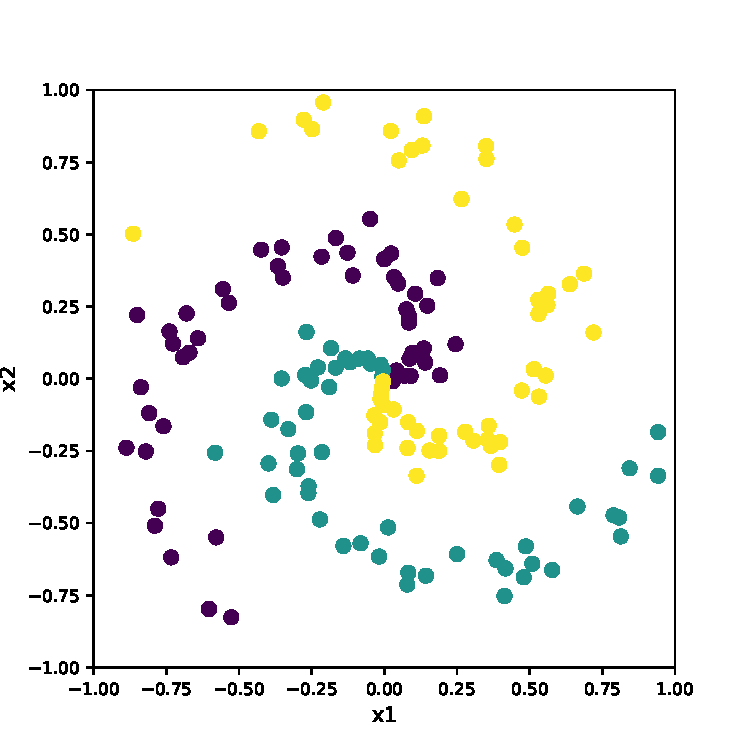
\includegraphics[width=8.1cm]{spiral_data.pdf}
\end{center}
For each datapoint $\mathbf{x} = (x_1, x_2)$, the label is the branch index such that $y = 0, 1$ or 2 for the example above.
Our goal is to implement a neural network capable of classifying the branches.

This network will compare its output with labels in the so-called \emph{one-hot encoding}.
For a given label \texttt{y=k}, the corresponding one-hot encoding is a \texttt{K}-dimensional vector with all entries zero 
except for the \texttt{k}$^\text{th}$ entry (which has value 1).
So when \texttt{K=3} the one-hot encodings for the labels are
\begin{equation*}
0 \rightarrow \begin{bmatrix} 1 \\ 0 \\ 0 \end{bmatrix}, \qquad
1 \rightarrow \begin{bmatrix} 0 \\ 1 \\ 0 \end{bmatrix}, \qquad
2 \rightarrow \begin{bmatrix} 0 \\ 0 \\ 1 \end{bmatrix}.
\end{equation*}

The code first defines the structure of the neural network 
and then uses the dataset to train this network.
The code generates two files: \texttt{spiral{\textunderscore}data.pdf} (a plot of the dataset such as the one above)
and \texttt{spiral{\textunderscore}results.pdf} (which displays three plots illustrating the results of training).

%%%%%%%%%%%%%%%%%%%%%%%%%%%%%%
%%%%%%%%%%%%%% Q1 %%%%%%%%%%%%%%
%%%%%%%%%%%%%%%%%%%%%%%%%%%%%%
\section{Neural network architecture, activation functions, cost functions and learning rate}

%\vspace{-2mm}Use the first part of the tutorial to do as many parts of this problem as you can.
%After 45 minutes, Lauren will email out the solution to part c), which will be needed to proceed to Problem 2.

%\opt{soln}{\newpage}
\begin{enumerate}[label=\alph*)]

%%%%%%%%%%%%%% (a) %%%%%%%%%%%%%%
\item Run the code and look at how it attempts to classify the two-dimensional space.
You should find that the resulting classifier separates the two-dimensional space using lines, 
and thus does a poor job of representing the data.

%%% SOLUTION %%%
\soln{Using the parameters provided (with the learning rate set to 1), you should find that the given network classifies the two-dimensional space as:
\begin{center}
\includegraphics[width=15.5cm, clip, trim=1.5cm 0 1.5cm 1.5cm]{Code/spiral_results_K3_LR1.pdf} %trim: Left, bottom, right, top
\end{center}

\note{If the learning rate is 0.001, you will be able to observe the training cost decreasing:
\begin{center}
\includegraphics[width=15.5cm, clip, trim=1.5cm 0 1.5cm 1.5cm]{Code/spiral_results_K3_LR0-001.pdf}
\end{center}
}
}

%%%%%%%%%%%%%% (b) %%%%%%%%%%%%%%
\opt{soln}{\newpage}
\item Look through the section of code marked \texttt{DEFINE THE NETWORK ARCHITECTURE}.
On paper, draw the neural network corresponding to the one in the code for the case of \texttt{K} branches. 
Pay particular attention to the number of neurons in each layer.

%%% SOLUTION %%%
\soln{The neural network for the given code is:
\begin{center}
\includegraphics[height=5cm]{1b_network.pdf}
\end{center}
where the last layer has $K$ neurons.
}

%%%%%%%%%%%%%% (c) %%%%%%%%%%%%%%
\item Add in a hidden layer with 4 neurons and study how this hidden layer changes the output. 
On paper, draw the neural network in this case.

%%% SOLUTION %%%
\soln{Replace the \texttt{Layer 1} and \texttt{Network output} sections with the following code:

\texttt{nH=4} \\
\texttt{\#\#\# Layer 1: \#\#\#} \\
\texttt{W1 = tf.Variable(tf.random{\textunderscore}normal([2, nH], mean=0.0, stddev=0.01, dtype=tf.float32))} \\
\texttt{b1 = tf.Variable( tf.zeros([nH]) )} \\
\texttt{z1 = tf.matmul(x, W1) + b1} \\
\texttt{a1 = tf.nn.sigmoid( z1 )} \\

\texttt{\#\#\# Layer 2: \#\#\#} \\
\texttt{W2 = tf.Variable(tf.random{\textunderscore}normal([nH, K], mean=0.0, stddev=0.01, dtype=tf.float32))} \\
\texttt{b2 = tf.Variable( tf.zeros([K]) )} \\
\texttt{z2 = tf.matmul(a1, W2) + b2} \\
\texttt{a2 = tf.nn.sigmoid( z2 )} \\

\texttt{\#\#\# Network output: \#\#\#} \\
\texttt{aL = a2} \\

\newpage
After adding a hidden layer with 4 neurons, the neural network is:
\begin{center}
\includegraphics[height=5cm]{1c_network.pdf}
\end{center}
where the last layer has $K$ neurons.
}

%%%%%%%%%%%%%% (d) %%%%%%%%%%%%%%
\item Replace the sigmoid activation function on the first layer with a rectified linear unit (ReLU), and study how the 
choice of activation function changes the output.

%%% SOLUTION %%%
\soln{Replace the line \texttt{a1 = tf.nn.sigmoid( z1 )} with:

\texttt{a1 = tf.nn.relu( z1 )}

When using the sigmoid activation function, you might observe that the classifier separates the two-dimensional space
into regions that meet roughly at the origin.
When using the ReLU activation function on the first layer, the meeting place for these regions tends to jump around more.}

%%%%%%%%%%%%%% (e) %%%%%%%%%%%%%%
\item Change the cost function so that it is computed using the mean-squared error (MSE) instead of the cross-entropy,
and study how the choice of cost function changes the output.

%%% SOLUTION %%%
\soln{Add the following beneath the line \texttt{cost{\textunderscore}func = cross{\textunderscore}entropy}:

\texttt{mse = tf.reduce{\textunderscore}mean( tf.reduce{\textunderscore}sum( tf.square(y{\textunderscore}onehot - aL) ) )} \\
\texttt{cost{\textunderscore}func = mse}
}

%%%%%%%%%%%%%% (f) %%%%%%%%%%%%%%
\item Study the effects of increasing and decreasing the \texttt{learning{\textunderscore}rate} hyperparameter.
Examine these effects using both the cross-entropy and mean-squared error cost functions.

%%% SOLUTION %%%
\soln{When using sigmoid activation functions and the mean-squared error as the cost function, for the given data set you will likely find that the network does not make progress when 
\texttt{learning{\textunderscore}rate=1.0}. Decreasing the learning rate to 0.1 enables the network to make progress.
For discussion about the affects of changing the learning rate, see Section IVA of \texttt{arXiv:1803.08823}.
}

%%%%%%%%%%%%%% (g) %%%%%%%%%%%%%%
\opt{soln}{\newpage}
\item Explain why the \texttt{K}-dimensional one-hot encoding is useful. What do you think would happen if you used a one-dimensional label (such that $\texttt{y}=0,1,\ldots, \texttt{K}=1$ or $\texttt{K}$) instead?

%%% SOLUTION %%%
\soln{As an illustrative example, consider the case where there are \texttt{K=3} branches and the network is uncertain about whether the datapoint $\mathbf{x}$ belongs to branch 0 or branch 2. 
Specifically, let's say that the network is
50\% sure that $\mathbf{x}$ belongs to branch 0 and 
50\% sure that it belongs to branch 2.
This situation is easy to express in terms of the one-hot encoding as
\begin{equation*}
\mathbf{a}^{(L)} = \begin{bmatrix} 0.5 \\ 0 \\ 0.5 \end{bmatrix}.
\end{equation*}
Using a one-dimensional encoding, the network would only return a single number between 0 and 2. In this case, it might return the average predicted label such that
\begin{equation*}
\mathbf{a}^{(L)} = \begin{bmatrix} \frac{0+2}{2} \end{bmatrix} = \begin{bmatrix} 1 \end{bmatrix},
\end{equation*}
which is the same as the output it would return if it was certain that $\mathbf{x}$ belongs to branch 1. 
Thus, we see that a one-dimensional encoding can give network outputs that are hard to interpret when the number of classes \texttt{K} is greater than 2.
}

\end{enumerate}

%%%%%%%%%%%%%%%%%%%%%%%%%%%%%%
%%%%%%%%%%%%%% Q2 %%%%%%%%%%%%%%
%%%%%%%%%%%%%%%%%%%%%%%%%%%%%%
%\opt{soln}{\newpage}
\opt{nosoln}{\vspace{8mm}}
\section{Group work}
\vspace{-2mm}For this part of the tutorial, you will work in groups to explore the capabilities of a feedforward neural network with one hidden layer.
Each group will plot the accuracy of the neural network as a function of some quantity $Q$ (a property of the network or the data).

For all plots, the accuracy should be measured once you are convinced that the network has converged, 
which means that you may need to adjust the \texttt{N{\textunderscore}epochs} parameter in order to run the code longer.
In some cases, you may also find it useful to adjust the learning rate as $Q$ is varied (in particular if you find that your network is getting stuck or if training is very slow for certain values of $Q$).

%At the end of the tutorial, send your most interesting results (as well as a list of your group members) to Lauren and they will be discussed during tomorrow's lecture.
Each group's task is to plot the accuracy of the neural network as a function of some quantity $Q$, where
\begin{itemize}
\item {\usekomafont{descriptionlabel}{Groups 1 \& 2:}} $Q = $ the number of neurons in the hidden layer
\item {\usekomafont{descriptionlabel}{Groups 3 \& 4:}} $Q = $ \texttt{mag{\textunderscore}noise} (the magnitude of noise in the data)
\item {\usekomafont{descriptionlabel}{Groups 5 \& 6:}} $Q = $ \texttt{K} (the number of different labels)
\end{itemize}

%%% SOLUTION %%%
\opt{soln}{\newpage}
\soln{
{\usekomafont{descriptionlabel}{Results from Groups 1 \& 2:}}
\begin{center}
%\includegraphics[height=7cm]{GroupResults/accuracy_vs_hiddenNeurons.pdf}
\end{center}

%\newpage
{\usekomafont{descriptionlabel}{Results from Groups 3 \& 4:}}
\begin{center}
%\includegraphics[height=6cm, clip, trim=9cm 10cm 3.5cm 2.5cm]{GroupResults/noise_vs_accuracy.pdf} %trim: Left, bottom, right, top
%\includegraphics[height=7cm]{GroupResults/Group4/DL_acc_vs_noise.png}
\end{center}

\newpage
{\usekomafont{descriptionlabel}{Results from Groups 5 \& 6:}} 
\begin{center}
%\includegraphics[height=7.5cm]{GroupResults/FNNaccuracy_vs_numbranches.png} \\
%\includegraphics[height=7.5cm]{GroupResults/acc_vs_branches/Acc_K_eta1.pdf}
\end{center}
}

\end{document}
